\section{Greed Is Good, but Sloth Is Better}

Your boss is sending you to attend a conference to network with other people in your industry. The conference consists of various events (which may be seminars, lunches, teambuilding events, etc.), with each event having a start and end time. There can be multiple events going on at once.

The catch is that you don't really like conferences and networking, so would prefer to attend as few events as possible. However, you don't want your boss to catch on that you're trying to attend fewer events, so you'd like to attend a set of events that conflicts with every other event that you could be attending -- that way, if your boss asks you why you didn't attend more events, you'll be able to tell her that you couldn't attend any other events due to scheduling conflicts. You also can't attend more than one event at a time, so you need to make sure that the events you select don't overlap with each other.

Formally, the conference events are given as an input list $V$, and each event $v_i$ is defined by a start time and finish time $(s_i, f_i)$. Your goal is to select the smallest subset of \textbf{non-overlapping} events such that every event in $V$ overlaps with at least one of your chosen events. An event $v_i = (1,4)$ overlaps with the event $v_j = (3,5)$ but not with the event $v_k = (4,6)$.

\begin{questions}
	\question[3] Your co-worker took CPSC 320, and he's noticed that this problem is \textbf{awfully} similar to one he encountered in an assignment on greedy algorithms... He therefore proposes the following greedy algorithm (slightly modified from the solutions for A2) for choosing conference events to attend:

	\begin{quote}
		If there are no events, return None. Otherwise, consider the event $v'$ with the earliest end time. Of the events that intersect with $v'$, add to the solution the event $v$ with the latest end time. Remove all events that intersect with $v$ and recurse on the remaining events.
	\end{quote}

	Give and briefly explain a counterexample in which this algorithm does not return an optimal solution.
	\ifsolutions\begin{soln}
	Let \(V\) be a vertex set. Add \(v \in V\). Then also add \(v_1, v_2, \dots, v_n\) to \(V\).

	Then for \(v_1, v_2, \dots, v_d\) add \((v, v_i) \in E\) for \(i = 1, 2, \dots, d\).

	Then colour the node \(v\) blue, and colour all other nodes in \(V\) red.

	By construction, the degree of all other nodes that are not \(v\) is \(1\) since it's only connected to \(v\).

	Thus, the degree of \(v\) is the maxmimum degree of the graph, which is \(d\).

	Since no nodes are adjacent except for ones to \(v\). Then the colour red is never shared by adjacent vertices.

	Thus, this graph with maximum degree \(d\) can be coloured with two colours.

\end{soln}
\fi

	\begin{soln}
		Consider the instance

		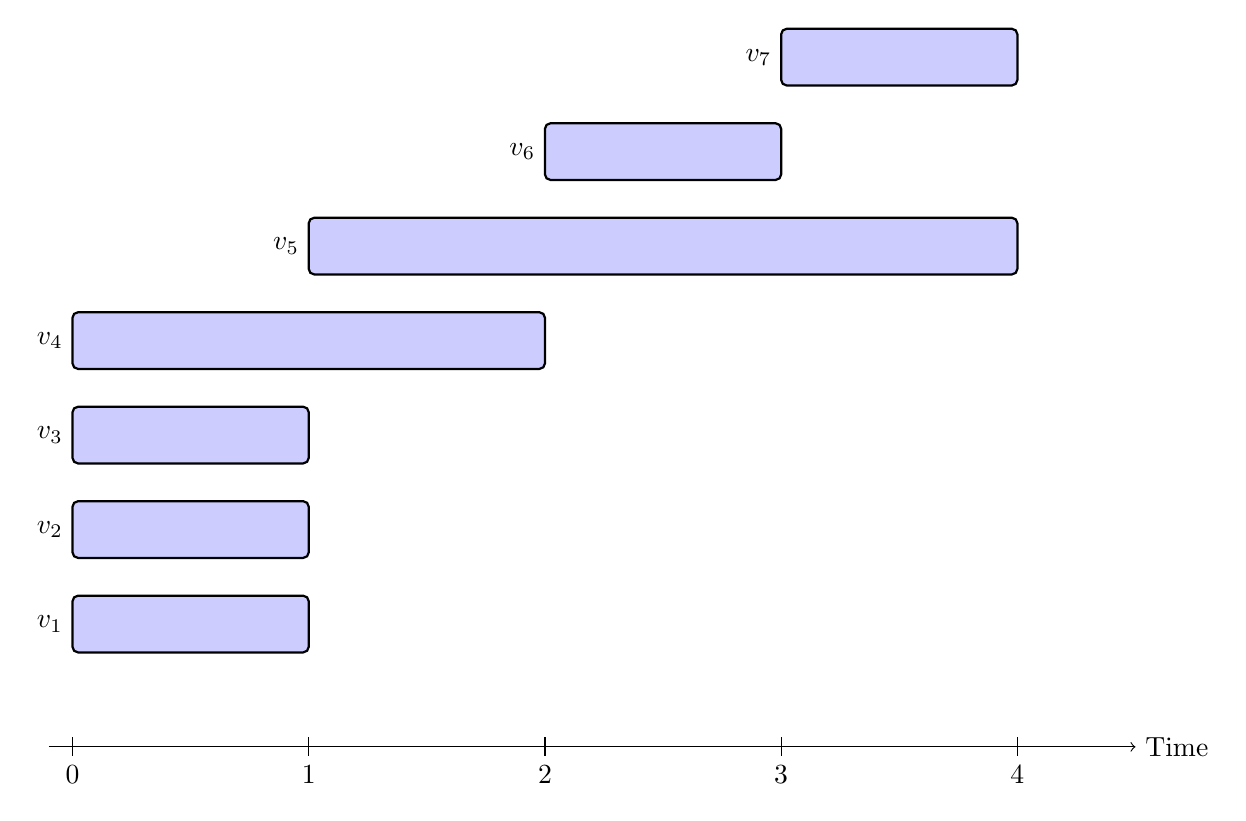
\begin{tikzpicture}[xscale=3, yscale=1.2]

			% Draw each interval as a blue bar with labels on the left
			\foreach \name/\start/\end/\y in {
					v_1/0/1/1,
					v_2/0/1/2,
					v_3/0/1/3,
					v_4/0/2/4,
					v_5/1/4/5,
					v_6/2/3/6,
					v_7/3/4/7
				} {
					\draw[thick, fill=blue!20, rounded corners=2pt] (\start,\y) rectangle (\end,\y+0.6);
					\node[left] at (\start,\y+0.3) {\(\name\)};
				}

			% Add axis labels
			\draw[->] (-0.1,0) -- (4.5,0) node[right] {Time};
			\foreach \x in {0,1,2,3,4} {
					\draw (\x,0.1) -- (\x,-0.1) node[below] {\x};
				}

		\end{tikzpicture}

		Using the proposed algorithm we would look at \(v_1\) and determine that \(v_4\) has the latest finish time such that it still intersects with \(v_1\).

		Thus, after removing all the events that intersect with \(v_4\) we are left with \(v_6\) and \(v_7\) that are disjoint, thus we would have to attned \(3\) events. In particular, we attned \(v_4, v_6, v_7\).

		However, if we select \(v_1\) and \(v_5\) we are able to intersect all of the events but by choosing one less event than proposed greedy would have.
	\end{soln}


	\question[4] Assume the events in $V$ are sorted by start time, and let $ME(i)$ denote the minimum number of events needed to cover events $i$ to $n$ (we say that an event is ``covered'' by a solution if it is either in the solution or overlaps with an event in the solution). Write a recurrence to define $ME(i)$.

	You can use the following helper function in your recurrence. For any index $i$, let $N(i)$ denote the index of the first event whose start time is greater than or equal to the end time of event $i$. You may assume that $N(i)$ is already implemented and that $N(i)$ returns $\infty$ if there are no events that begin after event $i$ ends.

	\ifsolutions\begin{soln}
	Proof: We provide a proof by induction on the number of nodes, \(n \in \mathbb{N}\), for graph \(G = (V, E)\).

	Base case \(|V| = 1\). The highest degree can be \(d = 0\), since the edge set would be empty.

	Thus, the algorithm uses \(1 = d + 1\) colours to colour the single node and the base case holds.

	Assume for any graph with \(n\) nodes that the algorithm will colour any ordering of nodes using at most \(d + 1\) colours.

	Consider a graph \(G = (V, E)\) with \(|V| = n + 1\) nodes with the highest degree of any node is \(d\).

	Let \(v_1, v_2, \dots, v_n, v_{n+1}\) be any ordering of the nodes. Remove \(v_{n+1}\) from this order, and the graph.

	Denote the deleted graph without \(v_{n+1}\) by \(G'\). Notice the degree of any node in \(G'\) can only decrease.

	Thus, the maximum degree of \(G'\) remains to be \(d\) with the removal of \(v_{n+1}\).

	By assumption, we can colour the ordering \(v_1, v_2, \dots, v_n\) using at most \(d+1\) colours.

	Since \(v_{n+1}\) has degree at most \(d\) then it has at most \(d\) neighbours. Then we add back \(v_{n+1}\).

	The number of colours used to colour its neigbours can be at most \(d\), if each are coloured distinctly.

	Thus, there remains at least \(1\) unique colour to colour \(v_{n+1}\) so that it is a valid colouring.

	In other words, the algorithm uses at most \(d + 1\) colours to colour the ordering \(v_1, v_2, \dots, v_{n+1}\).

	Induction makes the claim holds true for any graph with \(n\) nodes and maximum degree \(d\).


\end{soln}
\fi


	\begin{soln}
		For \(\{n\}\), we have no choice but to cover \(n\) using itself, so then \(ME(n) = 1\).

		If we consider some \(i < n\), either the optimal solution for \((i, i + 1, \dots, n)\) includes \(i\) or not.

		If it includes \(i\), then we must include into the optimal soltution the events that start after its finish time.

		Thus, we have that \(ME(i) = 1 + ME(N(i))\).

		In the case where where \(i\) is not included, then there is some later finishing event who intersects it and is part of the optimal solution.
		Without further information, its at least the next latest finishing event.
		If it includes \(i\), this means the other events in the solution do not intersect with \(i\).

		Thus it includes the events from the optimal solution from the event that starts after its finish time.

		Hence, \(ME(i) = 1 + ME(N(i))\).

		If it does not include \(i\), then there is some later starting event whose optimal solution covers \(i\).

		Such an event is at least the next starting event. Hence, \(ME(i) = ME(i + 1)\).

		Putting these together,

		\[
			ME(i) = \begin{cases}
				0            & \text{if } i > n            \\
				1            & \text{if } N(i) = \infty    \\
				1 + ME(N(i)) & \text{if } N(i) \neq \infty
			\end{cases}
		\]


	\end{soln}

	\question[4] Write pseudocode for an iterative dynamic programming algorithm to compute $ME(i)$ for all $i$ in $[1, \ldots, n]$.
	\ifsolutions\begin{soln}
	We consider the graph \(G = (V, E)\) with \(V = \{1, 2, 3, 4\}\) and \(E = \{(1, 4), (4, 3), (3, 2)\}\).

	\begin{center}
		\begin{tikzpicture}[node distance=2cm, auto]
			% Nodes
			\node[circle, draw, above  right = of 3] (1) {1};
			\node[circle, draw, right=of 1] (2) {2};
			\node[circle, draw, right=of 2] (3) {3};
			\node[circle, draw, above right=of 2] (4) {4};

			% Edges
			\draw (1) -- (4) -- (3) -- (2);
		\end{tikzpicture}
	\end{center}

	This graph can be coloured with three colours. Namely we can assign \(A = \{1, 3\}\) \(B = \{2, 4\}\).

	We see that no edges are shared between any vertices in \(A, B\) so this is a valid colouring.

	Now consider the ordering \(1, 2, 3, 4\). We first colour \(1\) blue. And then we consider \(2\).

	There is no edge between \(1, 2\) so we colour \(2\) blue and consider \(3\).

	So, its adjacent vertices have been coloured with blue, then we introduce a new colour for it red.

	Now we finally consider \(4\), its neighbours have been coloured with both red and green, so we must introduce a new colour for it purple.

	We have thus coloured this graph using three colours through the greedy algorithm when we could have used two.


\end{soln}
\fi
	\begin{soln}
		\begin{algorithmic}[1]
			\Procedure{MIN-EVENTS}{$n, N$}
			\State Define $ME[1 \dots n]$
			\State $i \gets n$
			\While {$i \geq 1$}
			\If {$N(i) = \infty$}
			\State $ME[i] = 1$
			\Else
			\State $ME[i] = 1 + ME[N[i]]$
			\EndIf
			\State $i := i - 1$
			\EndWhile
			\State \Return $ME[1]$
			\EndProcedure
		\end{algorithmic}
	\end{soln}


\end{questions}
